% Gemini theme
% https://github.com/anishathalye/gemini

% !TEX program = lualatex
\documentclass[final]{beamer}

% ====================
% Packages
% ====================

\usepackage[T1]{fontenc}
\usepackage{lmodern}
\usepackage[size=custom,width=36,height=48,scale=0.4]{beamerposter}
\usetheme{gemini}
\usecolortheme{mit}
\usepackage{graphicx}
\usepackage{booktabs}
\usepackage{tikz}
\usepackage{pgfplots}
\usepackage[capitalise]{cleveref}

% ====================
% Lengths
% ====================

% If you have N columns, choose \sepwidth and \colwidth such that
% (N+1)*\sepwidth + N*\colwidth = \paperwidth
\newlength{\sepwidth}
\newlength{\colwidth}
\setlength{\sepwidth}{0.02\paperwidth}
\setlength{\colwidth}{0.42\paperwidth}

\newcommand{\separatorcolumn}{\begin{column}{\sepwidth}\end{column}}


% Fix Beamer bibtex styling
\setbeamertemplate{bibliography entry article}{}
\setbeamertemplate{bibliography entry title}{}
\setbeamertemplate{bibliography entry location}{}
\setbeamertemplate{bibliography entry note}{}

% ====================
% Title
% ====================

\title{Assessment of Tethered Balloon-Borne Observations \\ of Arctic Low Cloud Properties}

\author{GUNHO (LOREN) OH \inst{1} \and SANGJONG PARK \inst{1}}

\institute[shortinst]{\inst{1} Korea Polar Research Institute (KOPRI)}

% ====================
% Footer (optional)
% ====================

\footercontent{
Korea Polar Research Institute (KOPRI), Incheon, Korea \hfill \null
}
% (can be left out to remove footer)

% ====================
% Logo (optional)
% ====================

% use this to include logos on the left and/or right side of the header:
% \logoright{\includegraphics[height=7cm]{logo1.pdf}}
% \logoleft{\includegraphics[height=7cm]{logo2.pdf}}

% ====================
% Body
% ====================

\begin{document}

\begin{frame}[t]
  \begin{columns}[t]

    \separatorcolumn
    \begin{column}{\colwidth}

      \begin{block}{Introduction}
        Low-altitude clouds exert a major influence on the radiative energy budget in the Arctic region. Studies have shown that Arctic clouds contribute to warming of the surface through long-wave cloud radiative effect, except during the peak of summer when the cooling effect due to their high albedo dominates. Although low-altitude clouds remain one of the largest uncertainties in modelling the Arctic climate, our understanding of the thermodynamic processes governing these clouds remains incomplete. In-situ observations of cloud properties are scarce, and uncertainties involved in remote sensing observations make it difficult to precisely determine the cloud properties and the thermodynamic state of the atmosphere. To this end, we make a comparison between an in-situ observation of the low-altitude clouds using a cloud particle detector, and measurements taken from a ground-based remote sensing site (retrieved from CloudNet). We examine the measurements taken from the Backscatter Cloud-probe with Polarization Detection (BCPD) mounted on a tethered balloon to obtain the cloud properties such as liquid water content (LWC), size-resolved number concentration (NC) and size distribution. The results from the  observation are used to examine the assumptions made in estimating the properties of the mixed-phase clouds from the remote sensor measurements.
      \end{block}

      \begin{block}{Methods}
        A Back-scatter Cloud Probe (BCPD) \cite{baumgardner2014ice, thomson2014compact} was mounted on a tethered balloon on October 1st, 2019, near Ny-\r{A}lesund, Svalbard, in order to make a set of observations on the thermodynamic and microphysical properties of low-altitude mixed-phase clouds. The instrument attached to the tethered balloon can be seen in \Cref{fig:01}.

        \begin{figure}
          \centering
          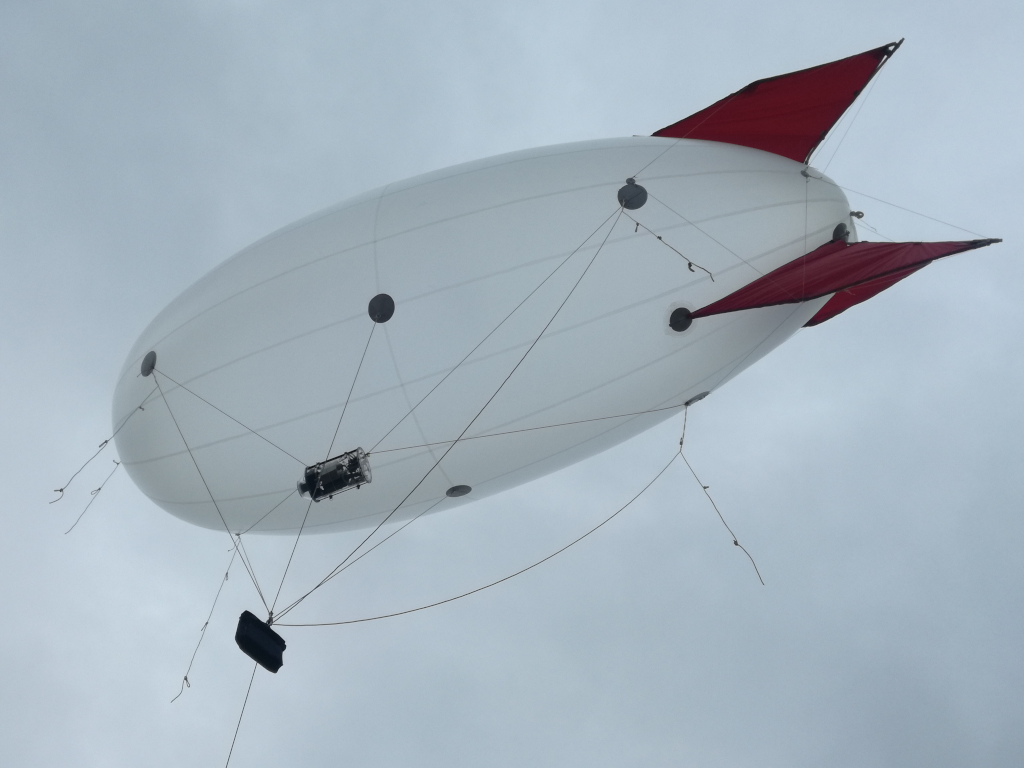
\includegraphics[width=0.8\colwidth]{figure/balloon.png}
          \caption{A photo of the Backscatter Cloud Probe (BCPD) mounted on a tethered balloon, deployed on October 1st, 2019 near Ny-\r{A}lesund, Svalbard.}
          \label{fig:01}
        \end{figure}
        
        The operation began at 18:00 UTC on October 1st, 2019, and lasted roughly two hours. The Back-scatter Cloud Probe (BCPD) measured a number of thermodynamic and microphysical properties of the advecting clouds at around 900 m above ground, with slightly varying altitude over time due to wind. The vertical trajectory of the instrument (and of the tethered balloon) can be seen in \Cref{fig:02} (black line). The sampled properties were processed into 10-second averages.

        We retrieved the liquid-water content (LWC) from ground-based remote sensing sites (Cloudnet) \cite{illingworth2007cloudnet}. The Cloudnet project provides vertical profiles of a number of cloud properties, which is useful for our study. The vertical profile of LWC is mapped in \Cref{fig:02}. By tracking the varying altitude of the tethered balloon and mapping the corresponding LWC values, we could compare the liquid-water content measured by BCPD against ground-based observations (\Cref{fig:05}). Although the cloudiness of the surrounding air remained fairly consistent (\emph{cf.} \Cref{fig:03}), the time-series of LWC reported by Cloudnet contains missing data, which is likely because clouds were not detected by the cloud radar at Ny-\r{A}lesund station \cite{illingworth2007cloudnet}. It is also possible that the presence of ice increased the uncertainty in the attenuation of ice reflectivity, but more work will be needed to estimate the properties of ice particles in the observed cloud.
        
        \begin{figure}
          \centering
          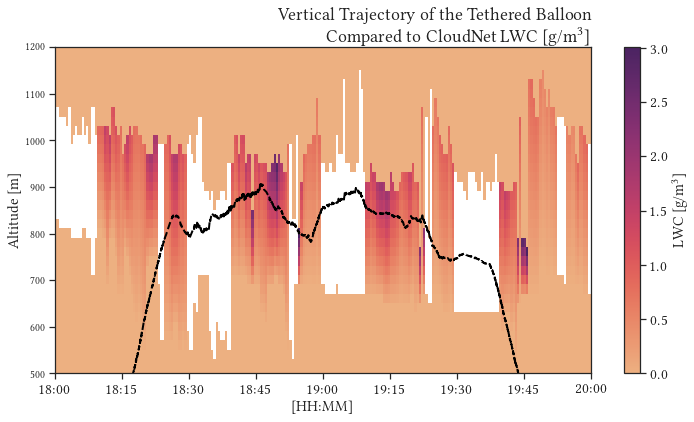
\includegraphics[width=\colwidth]{figure/ts_alt.png}
          \caption{The trajectory of the tethered balloon, compared to the liquid water content (LWC) in [g/m$^3$], reported by Cloudnet \cite{illingworth2007cloudnet}. The altitude recorded by the instrument on the tethered balloon is shown in black dashed line. The remotely-sensed LWC values are displayed on a coloured map, with white regions indicating gaps in the observation.}
          \label{fig:02}
        \end{figure}
      \end{block}
    \end{column}

    \separatorcolumn
    \begin{column}{\colwidth}

      \begin{block}{Results}
        \begin{figure}
          \centering
          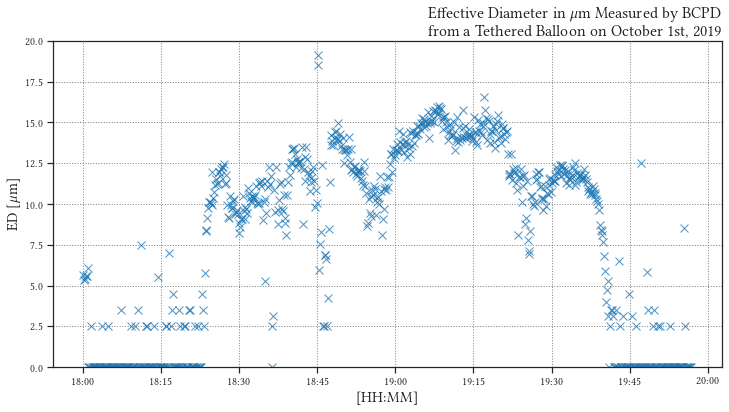
\includegraphics[width=\colwidth]{figure/ts_ed.png}
          \caption{A time-series plot of the effective diameter (in $\mu$) measured by BCPD mounted on a tethered balloon.}
          \label{fig:03}
        \end{figure}

        \begin{figure}
          \centering
          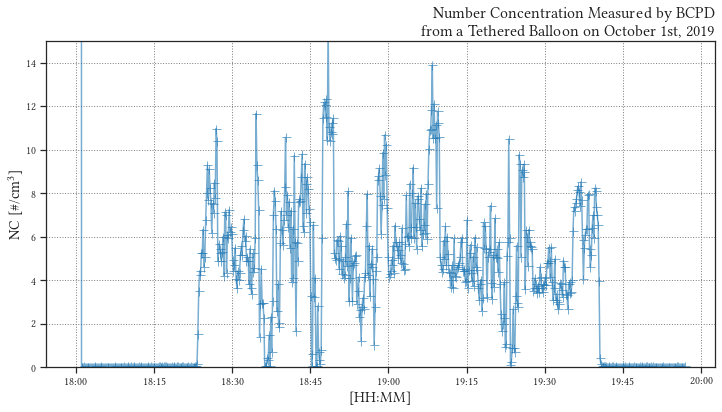
\includegraphics[width=\colwidth]{figure/ts_nc.png}
          \caption{A time-series plot of the number concentration (number of particles per cm$^3$) measured by BCPD mounted on a tethered balloon.}
          \label{fig:04}
        \end{figure}

        \begin{figure}
          \centering
          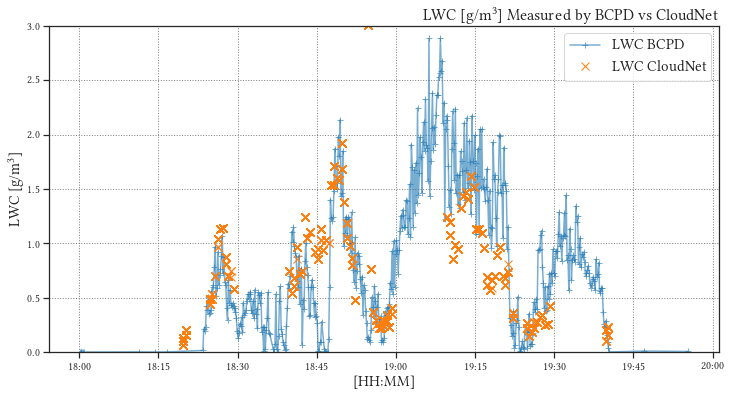
\includegraphics[width=\colwidth]{figure/ts_lwc.png}
          \caption{A time-series of the liquid water content (in g/m$^3$) measured by BCPD mounted on a tethered balloon (blue), compared to the values reported by the CloudNet remote-sensing observation (orange).}
          \label{fig:05}
        \end{figure}

      \end{block}

      \begin{block}{Conclusion}
        A preliminary analysis of the thermodynamic and microphysical properties of low-altitude, mixed-phase clouds measured by Back-scatter Cloud Probe (BCPD) \cite{baumgardner2014ice,thomson2014compact} reveals that the balloon-borne observation corresponds fairly well to ground-based remote-sensing data. The large variability in both the effective diameter (\emph{cf.} \Cref{fig:03}) as well as number concentration (\emph{cf.} \Cref{fig:04}) shows possible source of uncertainties in the measurements of cloud properties. 
        
        Further analysis is required to investigate the polarization ratio of the water droplets and ice particles observed by BCPD, which will provide more information about the microphysical characteristics of low-altitude, mixed-phase clouds in the Arctic region.
      \end{block}

      \begin{block}{References}
        \nocite{*}
        \footnotesize{\bibliographystyle{abbrv}\bibliography{poster}}
      \end{block}

    \end{column}

    \separatorcolumn
  \end{columns}

\end{frame}
\end{document}
